\documentclass{amsart}
\usepackage{amsmath,amssymb,latexsym}
\usepackage[margin=1in, marginparwidth=0.8in]{geometry}
\usepackage{tikz}

%%% discussion tools; remove this before publishing
\usepackage[draft]{say}
\newcommand{\sayDR}[1]{\say[DR]{#1}}
\newcommand{\sayLD}[1]{\say[LD]{#1}}
\newcommand{\sayPGP}[1]{\say[PGP]{#1}}
\newcommand{\sayPT}[1]{\say[PT]{#1}}
\newcommand{\saySS}[1]{\say[SS]{#1}}
%%% end discussion tools

\newtheorem{theorem}{Theorem}
\newtheorem{definition}[theorem]{Definition}
\newtheorem{corollary}[theorem]{Corollary}
\newtheorem{example}[theorem]{Example}
\newtheorem{lemma}[theorem]{Lemma}
\newtheorem{proposition}[theorem]{Proposition}
\newtheorem{remark}[theorem]{Remark}

\newcommand{\bepsilon}{\boldsymbol{\epsilon}}
\newcommand{\be}{\boldsymbol{e}}
\newcommand{\bi}{\boldsymbol{i}}
\newcommand{\fsl}{\mathfrak{sl}}
\newcommand{\ZZ}{\mathbb{Z}}

\author[Demonet]{Laurent Demonet}
\address[Laurent Demonet]{Graduate School of Mathematics, Nagoya University, Furocho, Chikusaku, 464-8602 Nagoya, Japan}
\email{Laurent.Demonet@normalesup.org}

\author[Plamondon]{Pierre-Guy Plamondon}
\address[Pierre-Guy Plamondon]{Laboratoire de Math\'ematiques d'Orsay, Univ. Paris-Sud, CNRS, Univ.
Paris-Saclay, 91405 Orsay, France.}
\email{pierre-guy.plamondon@math.u-psud.fr}

\author[Rupel]{Dylan Rupel}
\address[Dylan Rupel]{Department of Mathematics, University of Notre Dame, Notre Dame, Indiana 46556, USA.}
\email{drupel@nd.edu}

\author[Stella]{Salvatore Stella}
\address[Salvatore Stella]{IN$d$AM - Marie Curie Actions fellow, Universit\`a ``La Sapienza'', Roma, Italy.}
\email{stella@mat.uniroma1.it}

\author[Tumarkin]{Pavel Tumarkin}
\address[Pavel Tumarkin]{Department of Mathematical Sciences, Durham University, South Road, Durham, DH1 3LE, UK.}
\email{pavel.tumarkin@durham.ac.uk}


\title{$\fsl_2$-Tilings Do Not Exist in Higher Dimensions (mostly)}

\begin{document}
\begin{abstract}
  We show that there exists essentially a unique $\bepsilon$-$\fsl_2$-tiling, the anti-$\fsl_2$-tiling, and no $\fsl_2$-tilings in dimension bigger or equal to 3.
\end{abstract}
\maketitle

\section{$\fsl_2$-Tilings of the Plane}
  The aim of this note is to study higher-dimensional analogues of the following object.
  \begin{definition}[\cite{AssemReutenauerSmith}]
    A bi-infinite array $(a_{ij})_{i,j\in\ZZ}$ with $a_{ij}\in\ZZ_{>0}$ is called an \emph{$\fsl_2$-tiling of $\ZZ^2$} if the entries satisfy the relation
    \begin{equation}\label{eq:sl2 recursion}
      a_{i,j+1}a_{i+1,j}-a_{ij}a_{i+1,j+1}=1.
    \end{equation}
    A bi-infinite array $(b_{ij})_{i,j\in\ZZ}$ with $b_{ij}\in\ZZ_{>0}$  is called an \emph{anti-$\fsl_2$-tiling of $\ZZ^2$} if the entries satisfy the relation
    \begin{equation}\label{eq:anti-sl2 recursion}
      b_{i,j+1}b_{i+1,j}-b_{ij}b_{i+1,j+1}=-1.
    \end{equation}
  \end{definition}
  The notion of an anti-$\fsl_2$-tiling is not actually giving anything new as shown by the following lemma, however this notion will be useful for our considerations in higher dimensions.
  \begin{lemma}
    If $(a_{ij})_{i,j\in\ZZ}$ is an $\fsl_2$-tiling, then taking $b_{ij}=a_{i,-j}$ gives an anti-$\fsl_2$-tiling.
  \end{lemma}
  One should think of the difference between $\fsl_2$-tilings and anti-$\fsl_2$-tilings as viewing the lattice $\ZZ^2$ ``from above'' or ``from below.''

  The following result from \cite{AssemReutenauerSmith} was our starting point.
  \begin{theorem}[\cite{AssemReutenauerSmith}]
    There exist infinitely many $\fsl_2$-tilings of $\ZZ^2$.
  \end{theorem}

  In fact, it is shown in \cite{AssemReutenauerSmith} that any ``frontier'', or broken line of $1$'s in the plane, can be completed into a unique $\fsl_2$-tiling.
  An interpretation of all possible $\fsl_2$-tilings involving triangulations of a polygon with infinitely many vertices was later given in \cite{HolmJorgensen}.

  The following $\fsl_2$-tiling will be relevant in our higher dimensional analysis.
  \saySS{Do you think it could make more sense to make this into an anti-tiling example?}
  \sayPGP{Either way is fine for me.}
  \begin{example}\label{ex:Fibonacci}
    Consider the $\fsl_2$-tiling $(a_{ij})_{i,j\in\ZZ}$ of $\ZZ^2$ with $a_{ij}=1$ if $i-j\in\{0,1\}$.  
    Then using \eqref{eq:sl2 recursion} and the well-known recursion $F_{2r-1}F_{2r+3}=F_{2r+1}^2+1$ $(r\ge1)$ for the odd Fibonacci numbers, we see that
      \[
        a_{ij}
        =
        \begin{cases}
          F_{2r-1} & \text{if $i-j=r\ge1$;}\\
          F_{-2r+1} & \text{if $i-j=r\le0$;}
        \end{cases}
      \]
      where we number the Fibonacci numbers as:
      \[
        \begin{tabular}{|c|c|c|c|c|c|c|c} 
          $F_1$ & $F_2$ & $F_3$ & $F_4$ & $F_5$ & $F_6$ & $F_7$ & $\cdots$\\
          \hline 1 & 1 & 2 & 3 & 5 & 8 & 13 & $\cdots$
        \end{tabular}
      \]
      The following figure is a section of this tiling. 
      Note the bolded frontier of $1$'s; it is an ``infinite staircase''.
      \begin{center}
        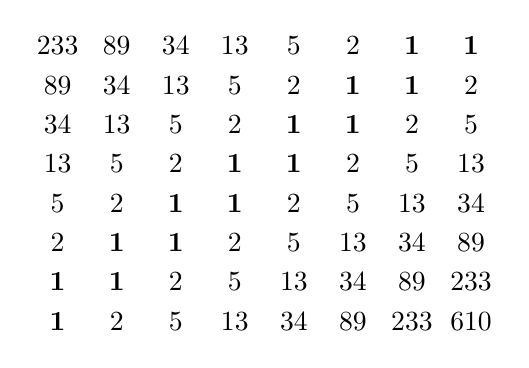
\begin{tikzpicture}
          \draw (0,1) node{$233$} (.75,1) node{$89$} (1.5,1) node{$34$} (2.25,1) node{$13$} (3,1) node{$5$} (3.75,1) node{$2$} (4.5,1) node{${\bf 1}$} (5.25,1) node{${\bf 1}$};
          \draw (0,.5) node{$89$} (.75,.5) node{$34$} (1.5,0.5) node{$13$} (2.25,0.5) node{$5$} (3,0.5) node{$2$} (3.75,0.5) node{${\bf 1}$} (4.5,0.5) node{${\bf 1}$} (5.25,0.5) node{$2$};
          \draw (0,0) node{$34$} (.75,0) node{$13$} (1.5,0) node{$5$} (2.25,0) node{$2$} (3,0) node{${\bf 1}$} (3.75,0) node{${\bf 1}$} (4.5,0) node{$2$} (5.25,0) node{$5$};
          \draw (0,-.5) node{$13$} (.75,-.5) node{$5$} (1.5,-.5) node{$2$} (2.25,-.5) node{${\bf 1}$} (3,-.5) node{${\bf 1}$} (3.75,-.5) node{$2$} (4.5,-.5) node{$5$} (5.25,-.5) node{$13$};
          \draw (0,-1) node{$5$} (.75,-1) node{$2$} (1.5,-1) node{${\bf 1}$} (2.25,-1) node{${\bf 1}$} (3,-1) node{$2$} (3.75,-1) node{$5$} (4.5,-1) node{$13$} (5.25,-1) node{$34$};
          \draw (0,-1.5) node{$2$} (.75,-1.5) node{${\bf 1}$} (1.5,-1.5) node{${\bf 1}$} (2.25,-1.5) node{$2$} (3,-1.5) node{$5$} (3.75,-1.5) node{$13$} (4.5,-1.5) node{$34$} (5.25,-1.5) node{$89$};
          \draw (0,-2) node{${\bf 1}$} (.75,-2) node{${\bf 1}$} (1.5,-2) node{$2$} (2.25,-2) node{$5$} (3,-2) node{$13$} (3.75,-2) node{$34$} (4.5,-2) node{$89$} (5.25,-2) node{$233$};
          \draw (0,-2.5) node{${\bf 1}$} (.75,-2.5) node{$2$} (1.5,-2.5) node{$5$} (2.25,-2.5) node{$13$} (3,-2.5) node{$34$} (3.75,-2.5) node{$89$} (4.5,-2.5) node{$233$} (5.25,-2.5) node{$610$};
        \end{tikzpicture}
      \end{center}
    \end{example}

\section{$\fsl_2$-Tilings in Higher Dimensions}
  Denote integer vectors by $\bi=(i_1\dots,i_n)$ and by $\be_k$ the $k$-th unit vector.
  A \emph{signature matrix} is a symmetric $n\times n$ matrix $\bepsilon=(\epsilon_{k\ell})$ with $\epsilon_{k\ell}=\pm 1$ whenever $k\neq \ell$ and $\epsilon_{kk}=1$. 
  \begin{definition}
    Fix a signature matrix $\bepsilon$.  
    An array $(a_{\bi})_{\bi\in\ZZ^n}$ with $a_{\bi}\in\ZZ_{>0}$ is called an \emph{$\bepsilon-\fsl_2$-tiling of $\ZZ^n$} if for each $k < \neq\ell$\sayLD{to replace by $k \neq \ell$} we have
    \begin{equation}\label{eq:higher sl2 recursion}
      a_{\bi+\be_\ell}a_{\bi+\be_k}-a_{\bi}a_{\bi+\be_k+\be_\ell}=\epsilon_{k\ell}.
    \end{equation}
  \end{definition}
  The requirement on the diagonal entries of signature matrices might seem arbitrary right now because they do not play any role in the above definition; we will see later on that it is indeed a consistent choice.
  
  The situation is now different than the $n=2$ case, all the $\bepsilon$-$\fsl_2$-tilings are not necessarily equivalent, however there do remain relations among them.
  \begin{lemma}\label{le:flip}
    Let $\bepsilon=(\epsilon_{k\ell})$ be any signature matrix and write $\bepsilon^{(r)}=(\epsilon'_{k\ell})$ where $\epsilon'_{k\ell}=-\epsilon_{k\ell}$ if $k=r$ or $\ell=r$ \sayPT{One probably needs $k\ne\ell$ here} and $\epsilon'_{k\ell}=\epsilon_{k\ell}$ otherwise. 
    Clearly $\bepsilon^{(r)}$ is a signature matrix.
    If $(a_{\bi})_{\bi\in\ZZ^n}$ is an $\bepsilon-\fsl_2$-tiling, then taking $b_{\bi}=a_{\bi-2i_r\be_r}$ gives an $\bepsilon^{(r)}-\fsl_2$-tiling.
  \end{lemma}

  \begin{definition}
    Let $\bepsilon$ be the signature matrix such that $\epsilon_{k\ell}=1$ (resp. $\epsilon_{k\ell}=-1$) whenever $k<\ell$.
\sayPT{$k\ne\ell$ means the same but looks better to me}
    We call any $\bepsilon$-$\fsl_2$-tiling an \emph{$\fsl_2$-tiling} (resp. \emph{anti-$\fsl_2$-tiling}) of $\ZZ^n$.
    \saySS{Do you have good name for these two matrices?}
  \end{definition}

  \begin{lemma}\label{le:constant slices}
    \sayLD{add something like: Suppose that $n \geq 3$.} Assume $(a_{\bi})_{\bi\in\ZZ^n}$ is either an $\fsl_2$-tiling or an anti-$\fsl_2$-tiling of $\ZZ^n$.
    Then for any $r\in\ZZ$ the set $\{a_{\bi}: \sum_{j=1}^n i_j=r\}$ consists of a single element.
  \end{lemma}
  \begin{proof}
    Pick any three distinct indices $j,k,\ell\in[1,n]$.
    To prove our claim we compute $a_{\bi+\be_j+\be_k+\be_\ell}$ in terms of $a_{\bi}, a_{\bi+\be_j}, a_{\bi+\be_k}, a_{\bi+\be_\ell}$ in three different ways.
    For simplicity of notation we set:
    \[
      a_{\bi}=a,
      \quad\quad 
      a_{\bi+\be_j}=x,
      \quad\quad 
      a_{\bi+\be_k}=y,
      \quad\quad 
      a_{\bi+\be_\ell}=z.
    \]
    The following picture will be useful.
    \begin{center}
      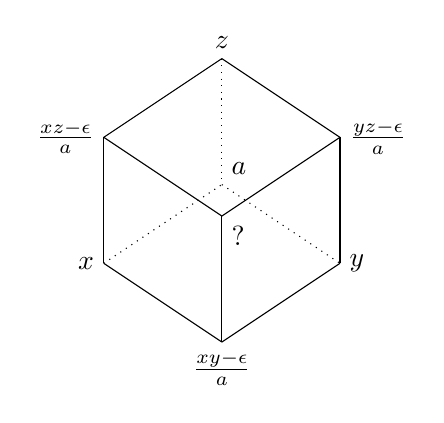
\begin{tikzpicture}
        \draw (0,0) -- ++(1.5,1)  node[above] {$z$} ;
        \draw (0,0) node[left] {$\frac{xz-\epsilon}{a}$} ;
        \draw (0,0) -- ++(0,-1.6) node[left] {$x$} ;
        \draw [dotted] (1.5,1) -- ++(0,-1.6) node[above right] {$a$};
        \draw [dotted] (0,-1.6) -- ++(1.5,1) ;
        \draw (0,0) -- ++(1.5,-1) node[below right] {?} ;
        \draw (1.5,1) -- ++(1.5,-1) node[right] {$\frac{yz-\epsilon}{a}$};
        \draw (0,-1.6) -- ++(1.5,-1) node[below]{$\frac{xy-\epsilon}{a}$};
        \draw [dotted] (1.5,-.6) -- ++(1.5,-1);
        \draw (1.5,-1) -- ++(0,-1.6) ;
        \draw (1.5,-1) -- ++(1.5,1) ;
        \draw (1.5,-2.6) -- ++(1.5,1) ;
        \draw (3,0) -- ++(0,-1.6) node[right]{$y$};
      \end{tikzpicture}
    \end{center}
    Using \eqref{eq:higher sl2 recursion} three times we get
    \[
      a_{\bi+\be_j+\be_k}=\frac{xy-\epsilon}{a},
      \quad\quad 
      a_{\bi+\be_k+\be_\ell}=\frac{yz-\epsilon}{a},
      \quad\quad 
      a_{\bi+\be_j+\be_\ell}=\frac{xz-\epsilon}{a}.
    \]
    Then applying \eqref{eq:higher sl2 recursion} three more times gives \sayLD{Replace all $\be_2$ by $\be_k$.}
    \begin{align*}
      a_{\bi+\be_j+\be_k+\be_\ell}
      &= \frac{a_{\bi+\be_j+\be_2}a_{\bi+\be_j+\be_\ell}-\epsilon}{a_{\bi+\be_j}}=\frac{xyz}{a^2}-\epsilon\frac{y+z}{a^2}-\epsilon\frac{a^2-\epsilon}{a^2x};\\
      &= \frac{a_{\bi+\be_j+\be_2}a_{\bi+\be_2+\be_\ell}-\epsilon}{a_{\bi+\be_2}}=\frac{xyz}{a^2}-\epsilon\frac{x+z}{a^2}-\epsilon\frac{a^2-\epsilon}{a^2y};\\
      &= \frac{a_{\bi+\be_j+\be_\ell}a_{\bi+\be_2+\be_\ell}-\epsilon}{a_{\bi+\be_\ell}}=\frac{xyz}{a^2}-\epsilon\frac{x+y}{a^2}-\epsilon\frac{a^2-\epsilon}{a^2z}.
    \end{align*}
    It follows that $\frac{x-y}{a^2}=\frac{a^2-\epsilon}{a^2x}-\frac{a^2-\epsilon}{a^2y}$ or $(xy+a^2-\epsilon)(x-y)=0$.  
    But $xy+a^2-\epsilon\ge1$ since $a,x,y\ge1$, hence $x=y$.  
    Similarly $y=z$.
    The result follows by iterating on all possible triples of distinct indices.
  \end{proof}

  We now come to our first main result: in dimension $n$, an ``infinite staircase'' of $1$'s yields the only possible anti-$\fsl_2$-tiling.

  \begin{theorem} \label{thm:antitiling} \sayLD{For $n \geq 3$, \dots}
    There exists a unique (up to translation) anti-$\fsl_2$-tiling of $\ZZ^n$. 
    Any of its ``two dimensional slices'' obtained by fixing all but two of the coordinates of $\bi$ is the unique anti-$\fsl_2$-tiling of $\ZZ^2$.
    In particular all the integers appearing are odd Fibonacci numbers.
    \saySS{Maybe phrasing here could be improved}
    \sayPT{In view of Theorem 3, ``the unique anti-$\fsl_2$-tiling of $\ZZ^2$'' looks a bit weird. It supposed to be the one with a staircase of 1's, right?}
    \sayLD{I propose to replace \emph{unique \dots} by \emph{staircase anti-$\fsl_2$-tiling} and we say before what it is}
  \end{theorem}  
  \begin{proof}
    Assume $(a_{\bi})_{\bi\in\ZZ^n}$ is a anti-$\fsl_2$-tiling of $\ZZ^n$.  
    Pick $\bi$ with $a_{\bi}$ minimal.  
    Applying \eqref{eq:higher sl2 recursion} gives
    \[
      a_{\bi+\be_1}a_{\bi-\be_2}=a_{\bi}a_{\bi+\be_1-\be_2}+1=a_{\bi}^2+1,
    \]
    where we applied Lemma~\ref{le:constant slices} in the last equality.
    If $a_{\bi}>1$, this implies $a_{\bi+\be_1}<a_{\bi}$ or $a_{\bi-\be_2}<a_{\bi}$, contradicting minimality, so we must have $a_{\bi}=1$.
    This implies $\{a_{\bi+\be_k},a_{\bi-\be_k}\}=\{1,2\}$.
\sayPT{Shouldn't this be $\{a_{\bi+\be_k},a_{\bi-\be_\ell}\}=\{1,2\}$, or it is essentially the same?} \sayLD{I propose to make it clearer to add before the sentence something like ``As $a_{\bi + \be_k}$ is independent of $k$, it implies for all $k$, \dots''}
    Without loss of generality we will assume $a_{\bi+\be_k}=2$ and $\sum_{j=1}^n i_j=1$.
    Then applying \eqref{eq:higher sl2 recursion} repeatedly shows that $a_{\bi'}$ with $\sum_{j=1}^n i'_j=r\ge1$ is exactly the $r^{th}$ odd Fibonacci number $F_{2r-1}$ (see Example~\ref{ex:Fibonacci}).
    Similarly one sees that $a_{\bi'}$ with $\sum_{j=1}^n i'_j =r\le0$ is the odd Fibonacci number $F_{-2r+1}$.
  \end{proof}

  \begin{proposition}\label{pr:nonexistence}
    There does not exist any $\fsl_2$-tiling of $\ZZ^n$ for $n\geq3$.
  \end{proposition}
  \begin{proof}
    It suffices to show that there is no $\fsl_2$-tiling of $\ZZ^3$.
    Assume $(a_{\bi})_{\bi\in\ZZ^3}$ is an $\fsl_2$-tiling of $\ZZ^3$.
    Pick $\bi$ with $a_{\bi}$ minimal.
    Applying \eqref{eq:higher sl2 recursion} gives
    \[
      a_{\bi+\be_1}a_{\bi-\be_2}=a_{\bi}a_{\bi+\be_1-\be_2}-1=a_{\bi}^2-1,
    \]
    where we applied Lemma~\ref{le:constant slices} in the last equality.
    But this implies $a_{\bi+\be_1}<a_{\bi}$ or $a_{\bi-\be_2}<a_{\bi}$, contradicting minimality.
  \end{proof}

  \begin{corollary}\label{co:n=3}
    For $n=3$, there are precisely $4$ matrices $\bepsilon$ for which there exists an $\bepsilon$-$\fsl_2$-tiling. 
    For such $\bepsilon$ this $\bepsilon$-$\fsl_2$-tiling is unique (up to translation).
    Moreover, if an $\bepsilon$-$\fsl_2$-tiling exists then $\epsilon_{12}\epsilon_{13}\epsilon_{23}=-1$.\sayLD{I propose to replace the last sentence by something like ``More precisely, an $\bepsilon$-$\fsl_2$-tiling exists if and only if $\epsilon_{12}\epsilon_{13}\epsilon_{23}=-1$'', or to change the phrasing to make appear the equivalence (it seems more interesting for me than the number)}
  \end{corollary}
  \begin{proof}
    The claim follows immediately from the observation that any signature matrix for $n=3$ either is one of the two satisfying $\epsilon_{12}=\epsilon_{13}=\epsilon_{23}$ or is obtained from one of these with a single application of Lemma~\ref{le:flip}.
  \end{proof}

  We are finally ready to classify all $\bepsilon$-$\fsl_2$-tilings for any $n\geq3$.
  \begin{theorem}
    There are precisely $2^{n-1}$ signature matrices $\bepsilon$ for which there exists an $\bepsilon$-$\fsl_2$-tiling of $\ZZ^n$ for $n\geq3$.
    They are all the signature matrices obtainable from the one yielding the anti-$\fsl_2$-tiling by repeated application of Lemma~\ref{le:flip}.
    Whenever an $\bepsilon$-$\fsl_2$-tiling exists it is unique up to translation.
  \end{theorem}
  \begin{proof} \sayLD{proof can be shortened (see after)}
    We will proceed by induction on $n$. 
    The base case, $n=3$, is the content of Corollary~\ref{co:n=3}.
    Observe that, if $(a_{\bi})_{\bi\in\ZZ^n}$ is an $\bepsilon$-$\fsl_2$-tiling of $\ZZ^n$, then all its slices $(a_{\bi})_{\bi\in\ZZ^n,i_n=r}$ are tilings of $\ZZ^{n-1}$.
    In particular, by the inductive hypothesis, $\bepsilon$ can be made into the matrix
    \[
      \bepsilon = 
      \left(
        \begin{array}{cccccc}
          1          & -1         & \cdots & -1             & -1             & \epsilon_1     \\
          -1         & 1          & \cdots & -1             & -1             & \epsilon_2     \\
          \vdots     & \vdots     & \ddots & \vdots         & \vdots         & \vdots          \\
          -1         & 1          & \cdots & 1              & -1             & \epsilon_{n-2} \\
          -1         & -1         & \cdots & -1             & 1              & \epsilon_{n-1} \\
          \epsilon_1 & \epsilon_2 & \cdots & \epsilon_{n-2} & \epsilon_{n-1} & 1
        \end{array}
      \right)
    \]
    by repeated application of Lemma~\ref{le:flip} in directions different from $n$.
    We claim now that, for an $\bepsilon$-$\fsl_2$-tiling of $\ZZ^n$ to exist, all the entries $\epsilon_j$ needs to be equal. 
    If not assume without loss of generality that $\epsilon_1 = -\epsilon_2 = -1$; then any slice of the corresponding $\bepsilon^{(1)}$-$\fsl_2$-tiling obtained fixing values for $i_4,\dots,i_n$ would be an $\fsl_2$-tiling of $\ZZ^3$ in contradiction with Proposition~\ref{pr:nonexistence}.
    Therefore all the $\epsilon_j$ coincide and either $\bepsilon$ or $\bepsilon^{(n)}$ yields the unique anti-$\fsl_2$-tiling of $\ZZ^n$.

    The counting of signature matrices giving raise to $\bepsilon$-$\fsl_2$-tilings follows immediately once one notices that 
    \[
      \left(\bepsilon^{(j)}\right)^{(k)}=\left(\bepsilon^{(k)}\right)^{(j)}
    \]
    for every $j,k\in[1,n]$ and that applying Lemma~\ref{le:flip} with $n$ distinct choices of $r$ fixes $\bepsilon$.
  \end{proof}
  \begin{proof}[Shorter proof]
   By Corollary \ref{co:n=3}, we get an inclusion $E \subset E'$ where $E$ is the set of signature matrices which admit a $\bepsilon$-$\fsl_2$-tiling and $E'$ is the set of signature matrices $\bepsilon$ satisfying $\bepsilon_{jk} \bepsilon_{k\ell} \bepsilon_{j\ell} = -1$ for any triple of indices $1 \leq j < k < \ell \leq n$. It is immediate that the restriction to any column (or row) gives a bijection from $E'$ to $\{\pm 1\}^{n-1}$. Using Lemma \ref{le:flip}, $(\ZZ/2\ZZ)^{n-1}$ acts on $E$ by $\bepsilon \mapsto \bepsilon^{(r)}$ for $1 \leq r \leq n-1$. By restricting the action to the last column of signature matrices, this action it free. Thanks to Theorem \ref{thm:antitiling}, $E$ is not empty so $\#E \geq 2^{n-1} = \# E' \geq \#E$ so $E = E'$. The unicity up to translation comes from restriction to triple of indices also.
  \end{proof}

  
  \begin{remark}
    It is now clear why we choose the diagonal entries of $\bepsilon$ to be equal to $1$: any $\bepsilon$-$\fsl_2$-tiling consists of odd Fibonacci numbers and each 1-dimensional slice satisfies \eqref{eq:higher sl2 recursion} with $k=\ell$.
  \end{remark} \sayLD{We could also remark that $2^{n-1}$ is the number of possible orientation of a $n$-staircase.}

\section*{Acknowledgements}
  These results were obtained while we were taking part in the Conference on Cluster Algebras and Representation Theory at the KIAS in Seoul, South Korea. 
  We would like to thank the organizers of that meeting for the stimulating environment they provided.

\begin{thebibliography}{99}
  \bibitem{AssemReutenauerSmith} Ibrahim Assem, Christophe Reutenauer and David Smith, \emph{Friezes}, Advances in Mathematics {\bf 225} (2010) 3134-3165.
  \bibitem{HolmJorgensen} Thorsten Holm and Peter J\o rgensen, \emph{To appear?}.
\end{thebibliography}

\end{document}
